
\chapter{Implementace a testování metod}

Praktická část práce se zabývá porovnáním výkonnosti jednotlivých
metod nalezení a popisu bodových příznaků na datasetu (JAK CITOVAT DATASET?)

Tento dataset sestává z jednotlivých subsetů obsahujících vždy několik obrázků
zobrazujících jednu scénu pod různými prostorovými transformacemi a porovnává se
vždy jeden z obrázků v subsetu s postupně všemi ostatními. Tyto transformace
lze popsat maticí homografie a dataset ke každému zkoumanému páru nabízí vzorovou
matici homografie.

Na tomto datasetu jsou zkoumány detektory příznakových bodů Harris, GFTT (neboli
Shi-Tomasi), SIFT, SURF, FAST, ORB a MSER a deskriptory BRIEF, SIFT, SURF a ORB.
Body nalezené a popsané těmito algoritmy jsou potom mezi jednotlivými obrazy
přiřazeny a metodou na bázi RANSAC je z nich aproximována matice homografie a 
jsou označeny body (páry bodů), které byly pro tuto aproximaci vzaty jako správné a ty, 
které byly zavrženy jako chybně přiřazené. 

%MĚŘÍTKO KVALITY NALEZENÉ HOMOGRAFIE

Jak bylo zmíněno, ke každému porovnávanému páru obrázků přísluší matice homografie,
která popisuje geometrickou transformaci mezi prvním a druhým obrázkem. Program
pomocí identifikace a spárovnání příznakových bodů s využitím metody RANSAC spočítá
odhad této homografie. Vzdálenost deklarované a nalezené homografie je potom brána
jako měřítko kvality konkrétní metody nebo kombinace metod na daném datasetu. Kvalita
homografie nabývá hodnot od 0 do 100% a vypočítává se jako:

\begin{equation}
	pi_1 = H_1 * eig(H_1) \\
	pi_2 = H_2 * eig(H_2) \\
	dif = pi_1 - pi_2 \\
	100*(\frac{pi}{2} - atan(dif \times{} 10^-4))
\end{equation}

kde $H_1$ je homografie deklarovaná v datasetu, $H_2$ je matice homografie nalezená
programem, $eig(H)$ jsou vlastní čísla matice $H$. 

Toto měřítko je v tabulkách ozančeno 'score'. Dále je zkoumán celkový počet přiřazených
bodů (označen 'matches') a z něj počet bodů použitých k aproximaci homografie (označen 'inliers').
Dále jsou zkoumány časy pro detekci a popis při použití jednotlivých detektorů a deskriptorů. 

%IMPLEMENTACE

Porovnání jednotlivých metod bylo implementováno v hlavním programu v C++ s využitím frameworku
openCV. Zpracování datasetu, dávkové spouštění porovnání a statistické vyhodnocení výsledků bylo
implementováno v jazyku Python s využitím knihovny Pandas.

%OBR: PSEUDOUML implementace

Data o souborech v datasetu jsou vytěžena pomocí skriptu \verb|create_configs.py| v Pythonu a zkompilována do konfiguračních souborů pro hlavní program BP. Skript \verb|run_batch.py| poté tyto konfigurační soubory načte a postupně s nimi spustí hlavní program. Ten pro každou vybranou složku datasetu vytvoří výstupní složku s obrázky, které zobrazují nalezené a spojené body mezi jedním a druhým obrázkem z vyhodnocovaného páru a soubor \verb|data.csv|, který obsahuje informace o jednotlivých párech, rychlostech vyhodnocení a kvalitě odhadu homografie. Skript \verb|get_data.py| ze souborů \verb|data.csv| vytvoří jeden globální soubor a několik souborů se subsety podle transformace, kterou reprezentují: Úhel (ve smyslu změna polohy pozorovatele směrem do stran), rotace (okolo osy procházející středem fotoaparátu), zoom, nasvětlení, rozostření a změna rozlišení. Tyto soubory jsou potom zpracovány skriptem\verb|pandas_stats.py| do obrázků a tabulek v této kapitole.

%PŘÍKLADY:

Ilustrační příklady nalezených a identifikovaných bodů:

\begin{figure}[htp] 
	\label{ex_asterix}
	\centering{
		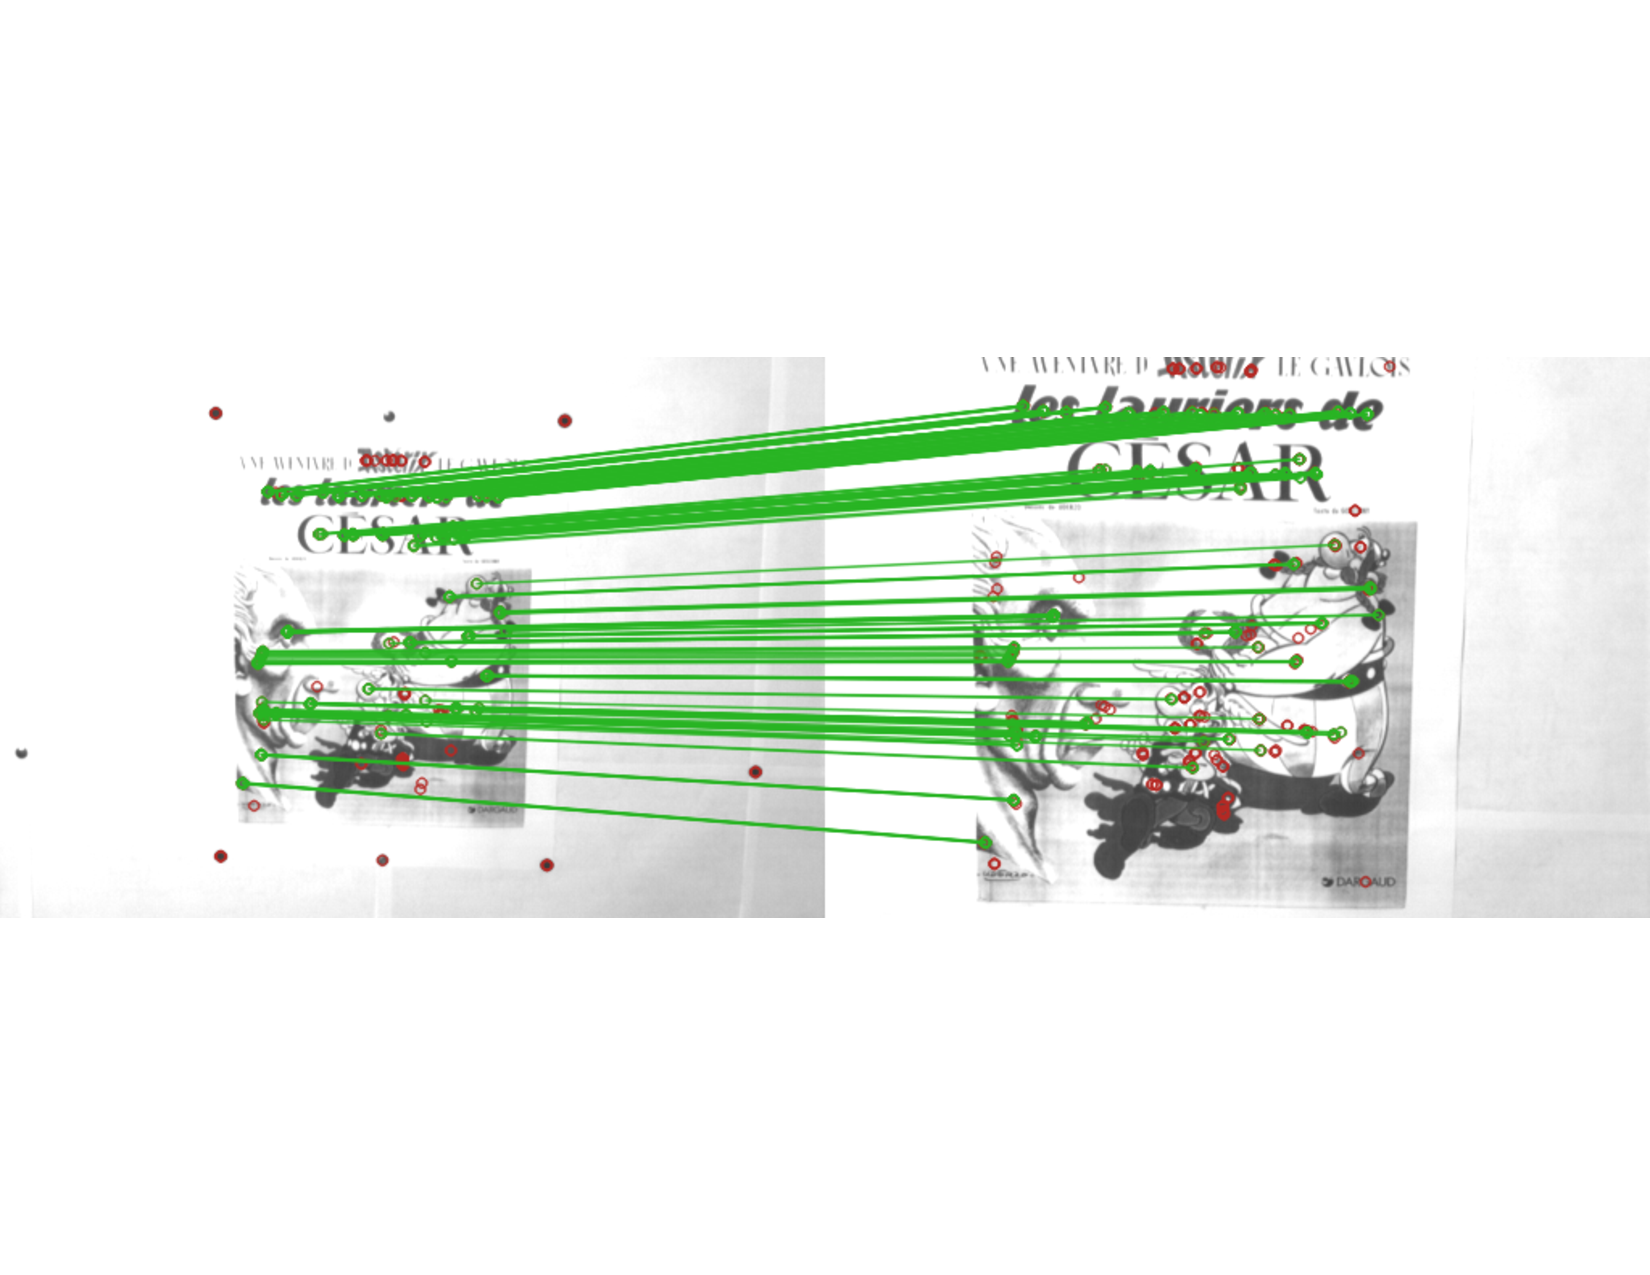
\includegraphics[scale=0.5]{text_img/ex_ASTERIX_MSER_SIFT.pdf}}
	\caption{Transformace zoom ze subsetu asterix, detektor MSER,
		deskriptor SIFT}
\end{figure}

\begin{figure}[htp] 
	\label{ex_belledonne}
	\centering{
		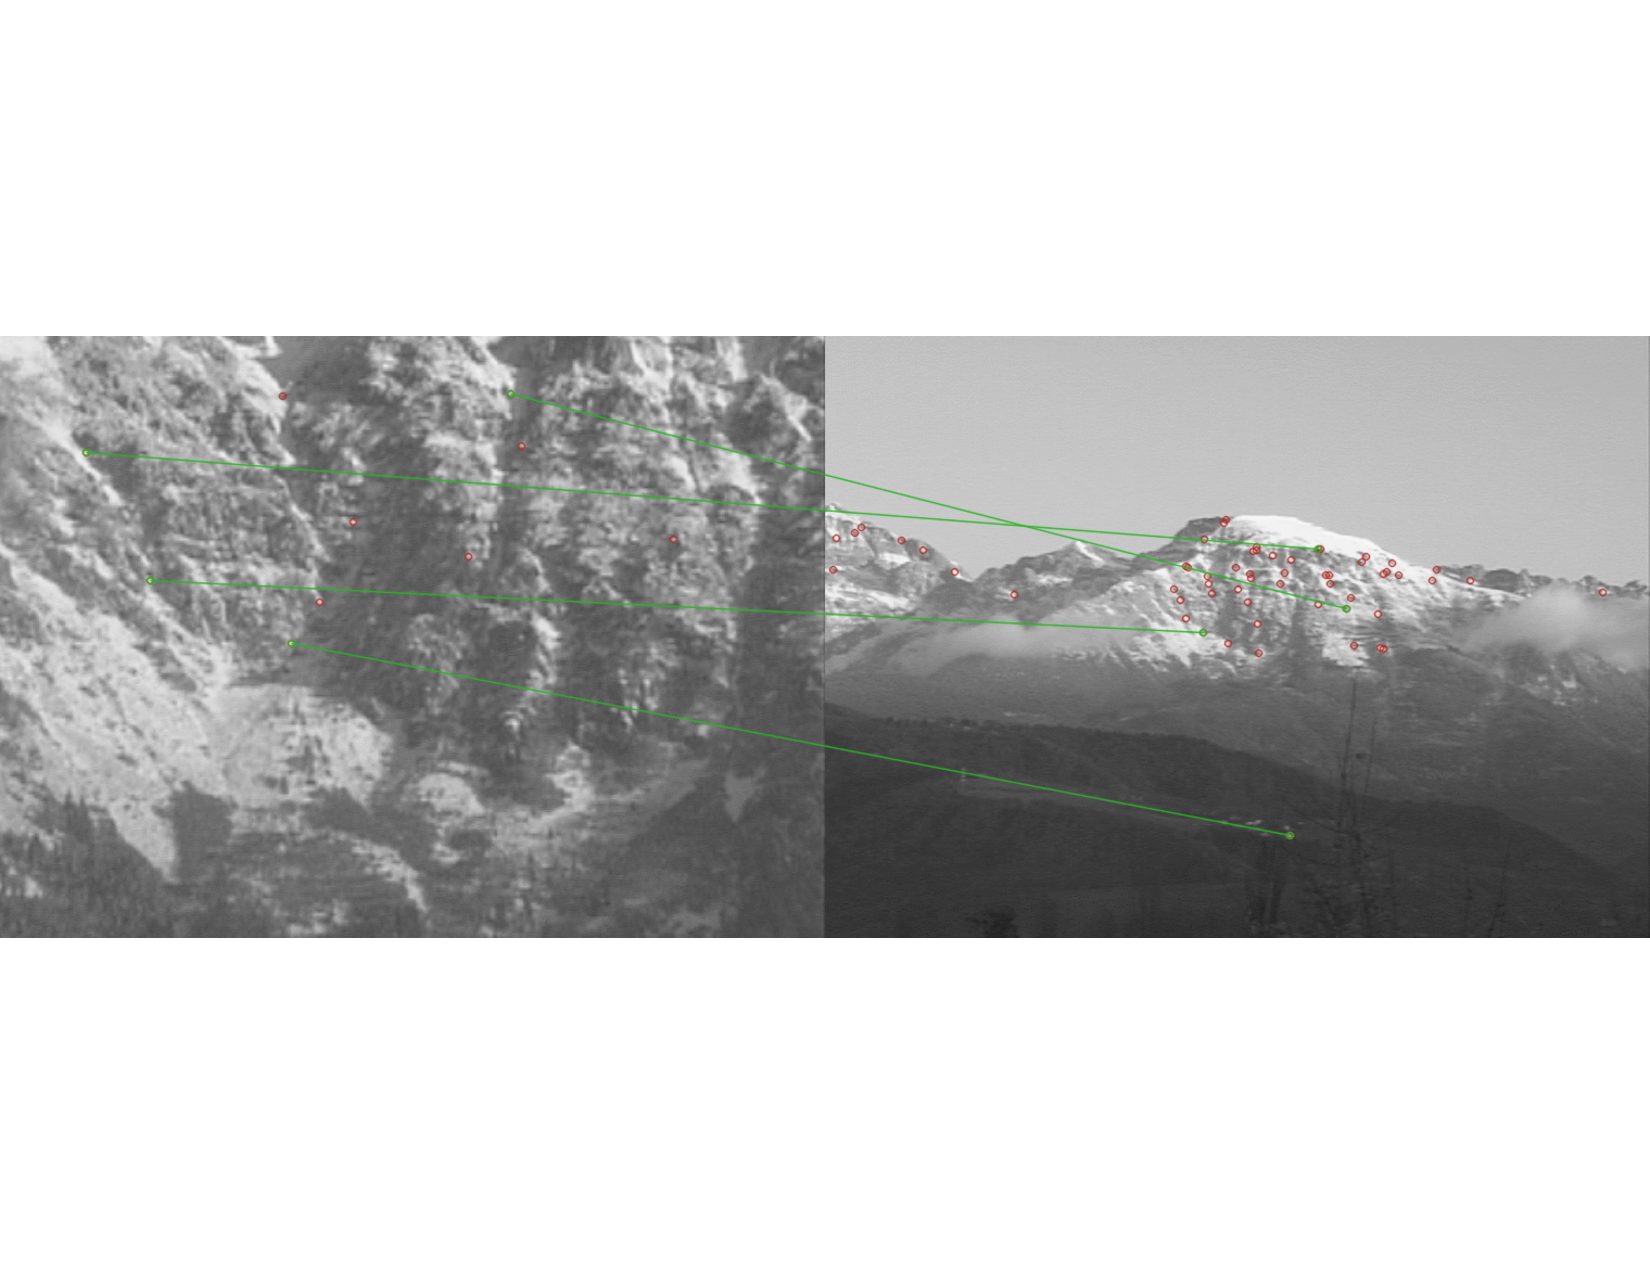
\includegraphics[scale=0.5]{text_img/ex_BELLEDONNE_FAST_ORB.pdf}}
	\caption{Ukázka transformace zoom ze subsetu belledonne, detektor FAST,
		deskriptor ORB}
\end{figure}

\begin{figure}[htp] 
	\label{ex_ensimag}
	\centering{
		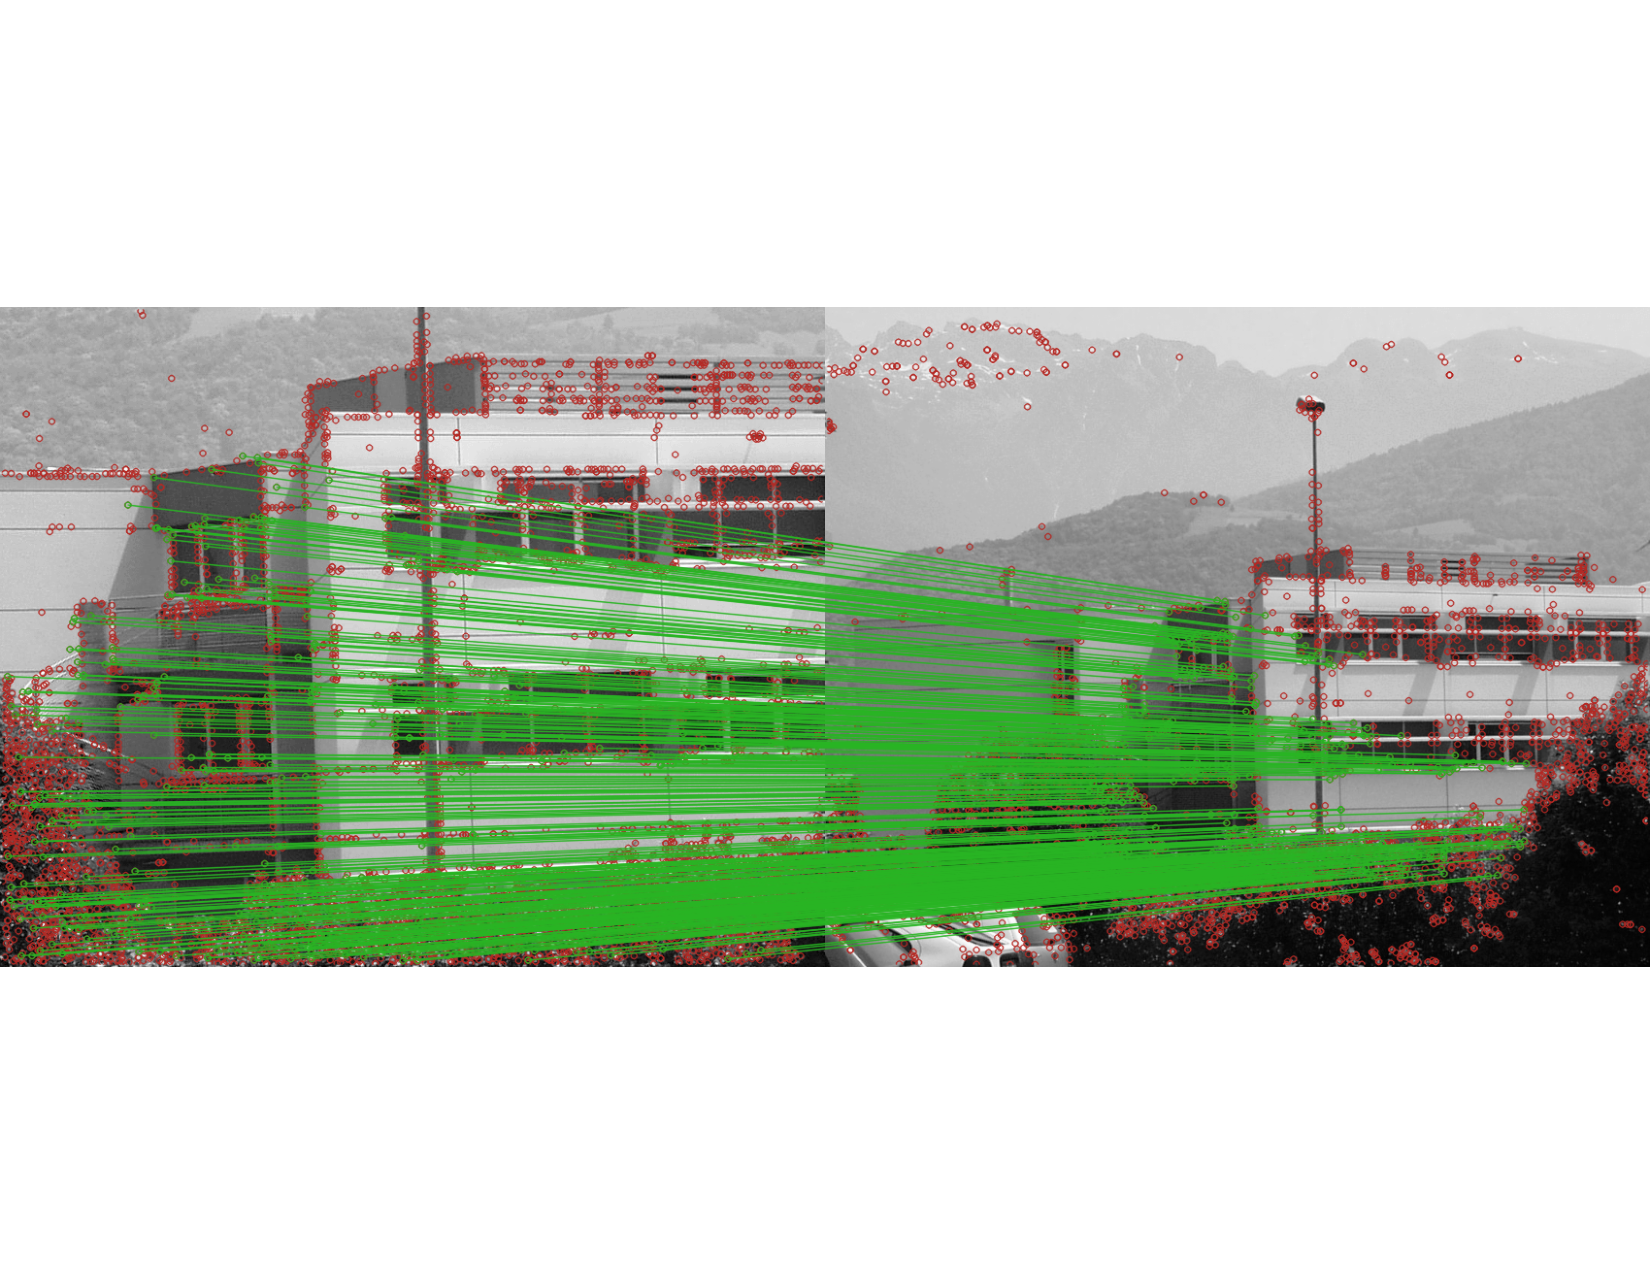
\includegraphics[scale=0.5]{text_img/ex_ENSIMAG_SIFT_SIFT.pdf}}
	\caption{Ukázka transformace zoom ze subsetu ensimag, detektor i 
		deskriptor SIFT}
\end{figure}

\begin{figure}[htp] 
	\label{ex_MONET}
	\centering{
		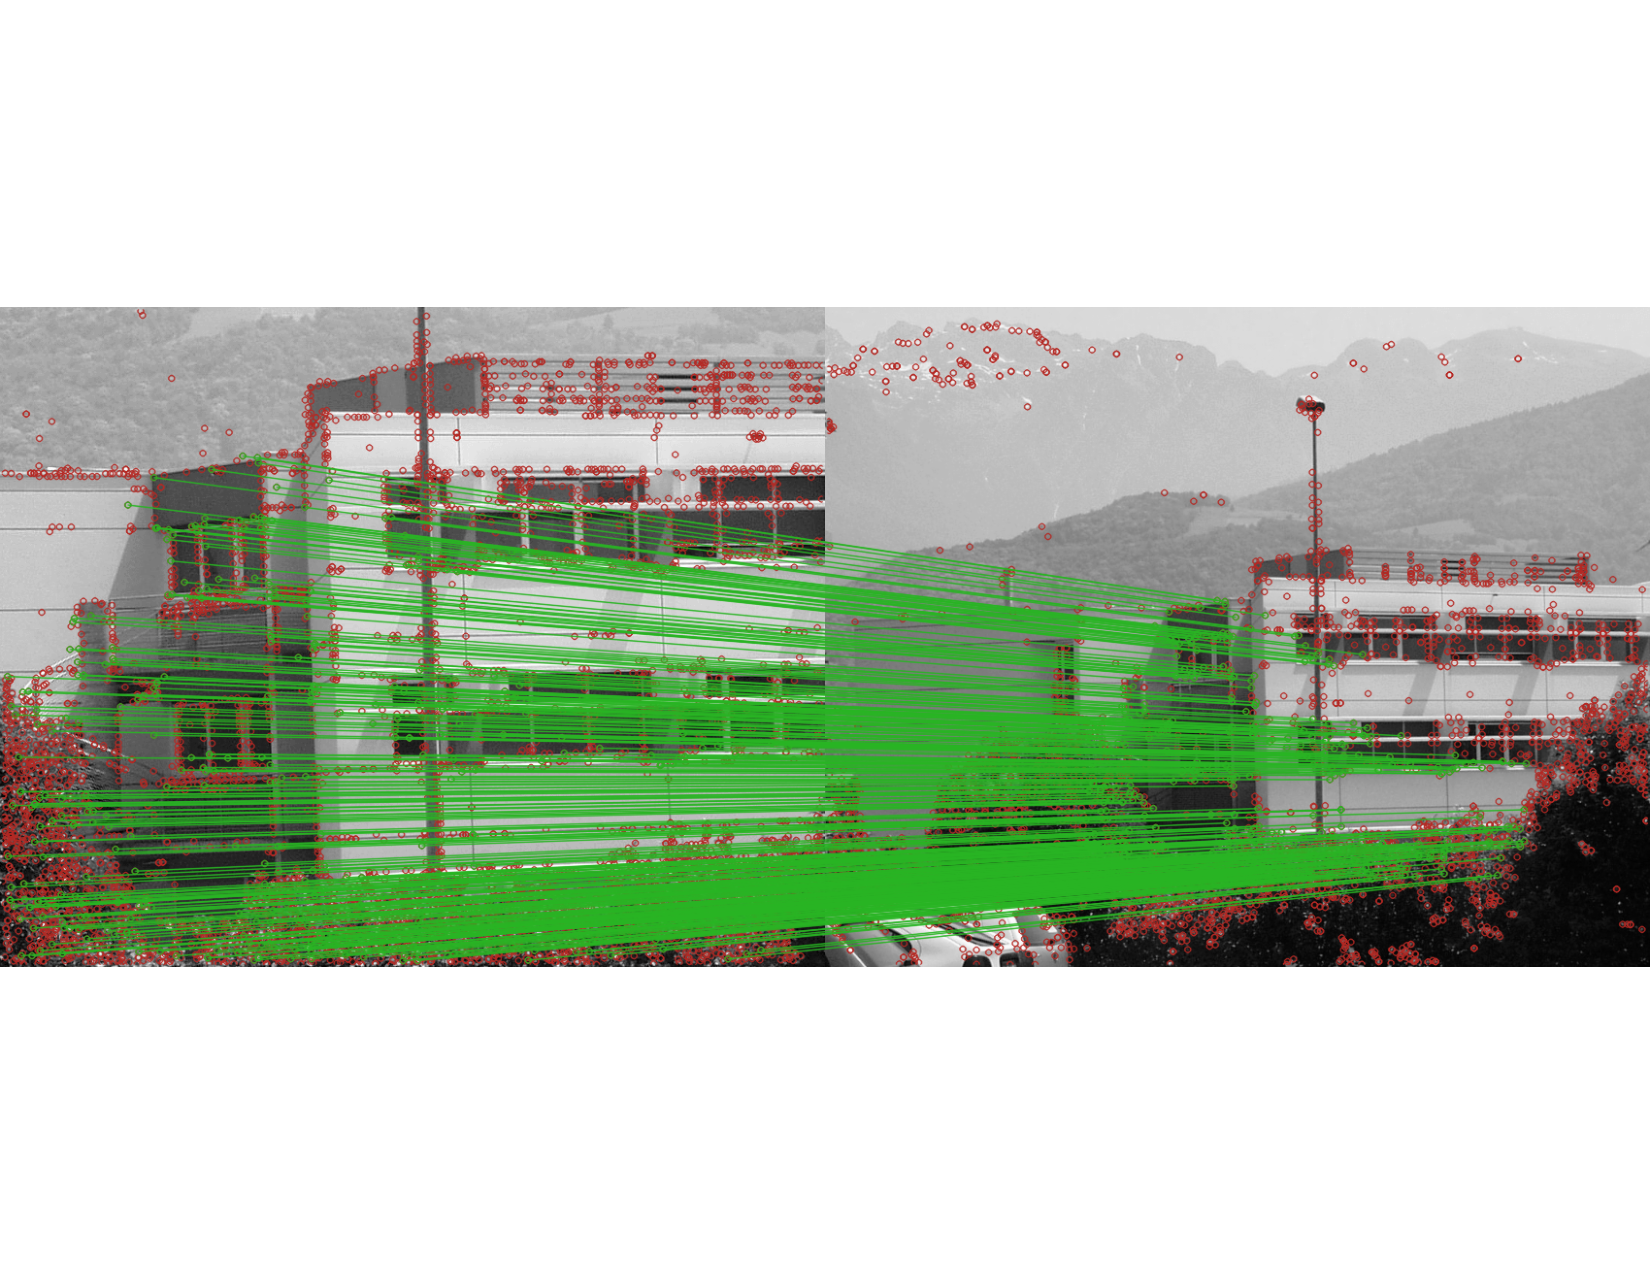
\includegraphics[scale=0.5]{text_img/ex_ENSIMAG_SIFT_SIFT.pdf}}
	\caption{Ukázka transformace rotace ze subsetu monet, detektor GFTT, 
		deskriptor SIFT}
\end{figure}

TABULKY:

výkonnost:

\begin{figure}[htp] 
	\label{det_perf}
	\centering{
		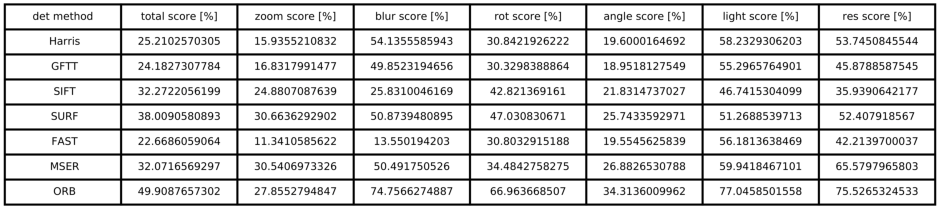
\includegraphics[scale=0.8]{text_img/Detector_performance.pdf}}
	\caption{Přehled výkonnosti detektorů na jednotlivých datasetech}
\end{figure}

\begin{figure}[htp] 
	\label{desc_perf}
	\centering{
		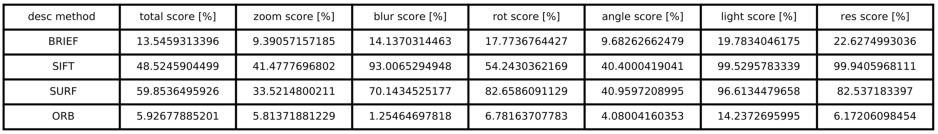
\includegraphics[scale=0.8]{text_img/Descriptor_performance.pdf}}
	\caption{Přehled výkonnosti deskriptorů na jednotlivých datasetech}
\end{figure}

\begin{figure}[h] 
	\label{det_desc_perf}
	\centering{}
		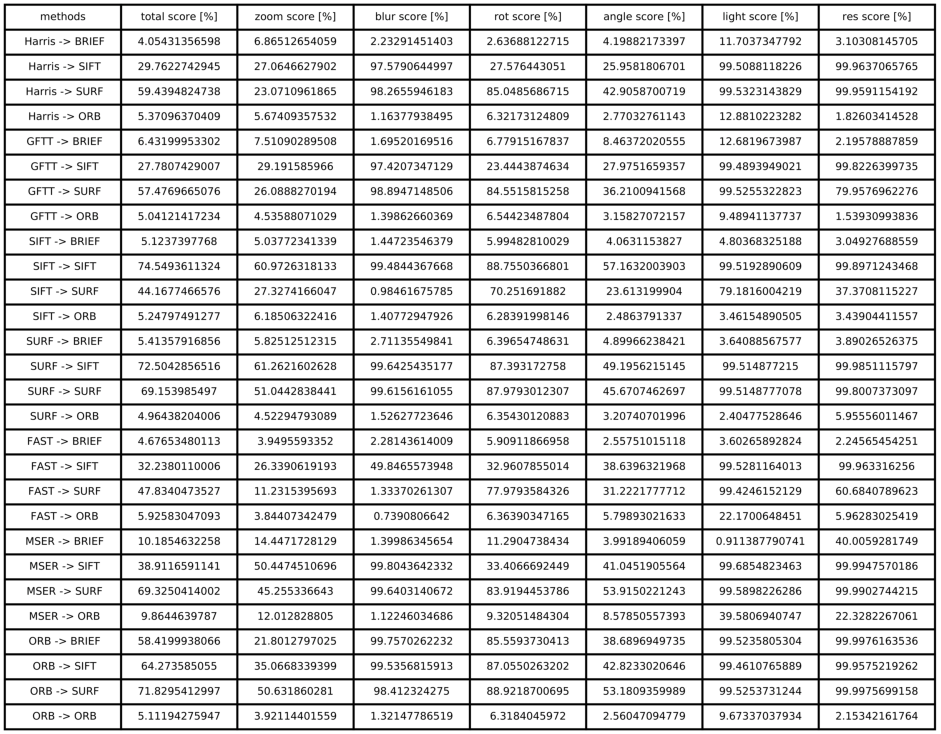
\includegraphics[scale=1]{text_img/Det_desc_perf.pdf}
	\caption{Přehled výkonnosti kobinací detektor->deskriptor na jednotlivých datasetech}
\end{figure}

časy: 

\begin{figure}[htp] 
	\label{det_times}
	\centering{
		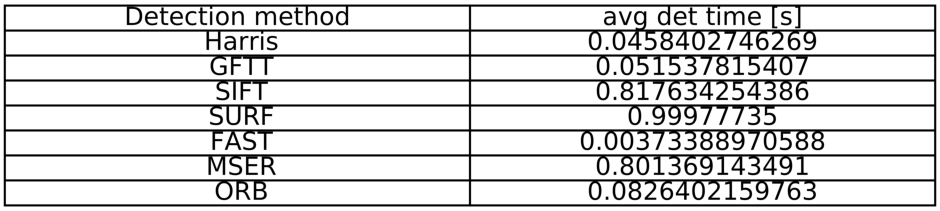
\includegraphics[scale=0.8]{text_img/Detection_times.pdf}}
	\caption{Přehled průměrné rychlosti detekce jednotlivými metodami ve vteřinách}
\end{figure}

\begin{figure}[htp] 
	\label{desc_times}
	\centering{
		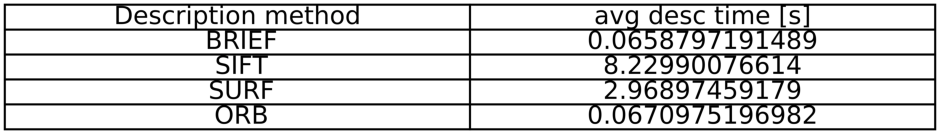
\includegraphics[scale=0.8]{text_img/Description_times.pdf}}
	\caption{Přehled průměrné rychlosti deskripce jednotlivými metodami ve vteřinách}
\end{figure}

počty:

\begin{figure}[htp] 
	\label{match_count}
	\centering{
		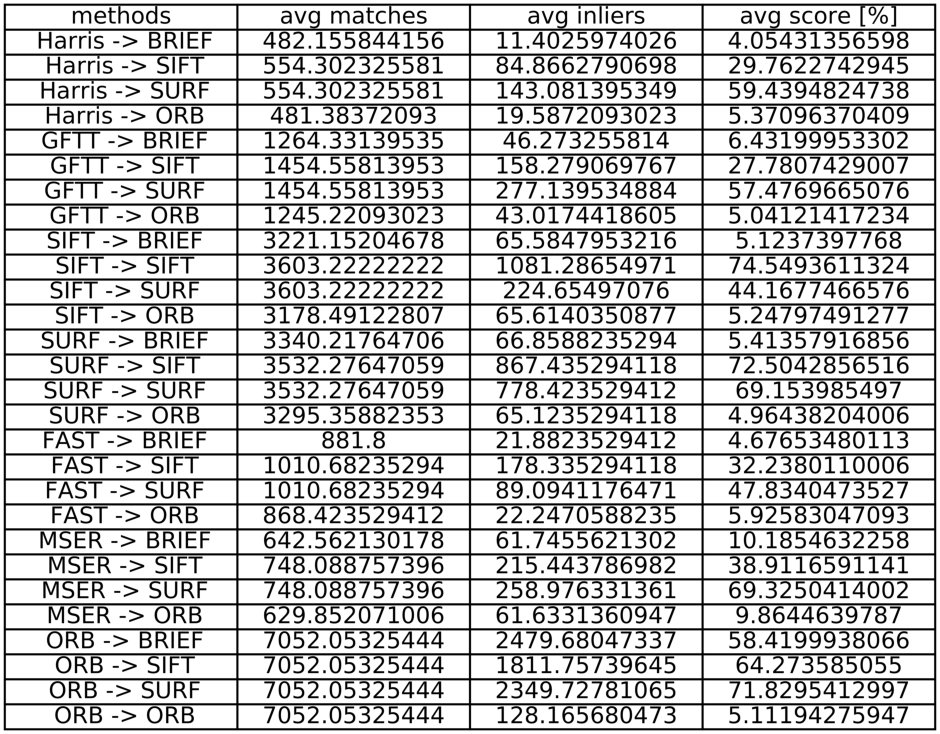
\includegraphics[scale=0.8]{text_img/Match_count.pdf}}
	\caption{Průměrné počty detekovaných a přiřazených příznaků jednotlivými kombinacemi metod}
\end{figure}

GRAFY

Vývoj kvality odhadu homografií jednotlivými kombinacemi metod na postupně více náročných
příkladech z jedné složky datasetu:

\begin{figure}[htp] 
	\label{graph_monet}
	\centering{
		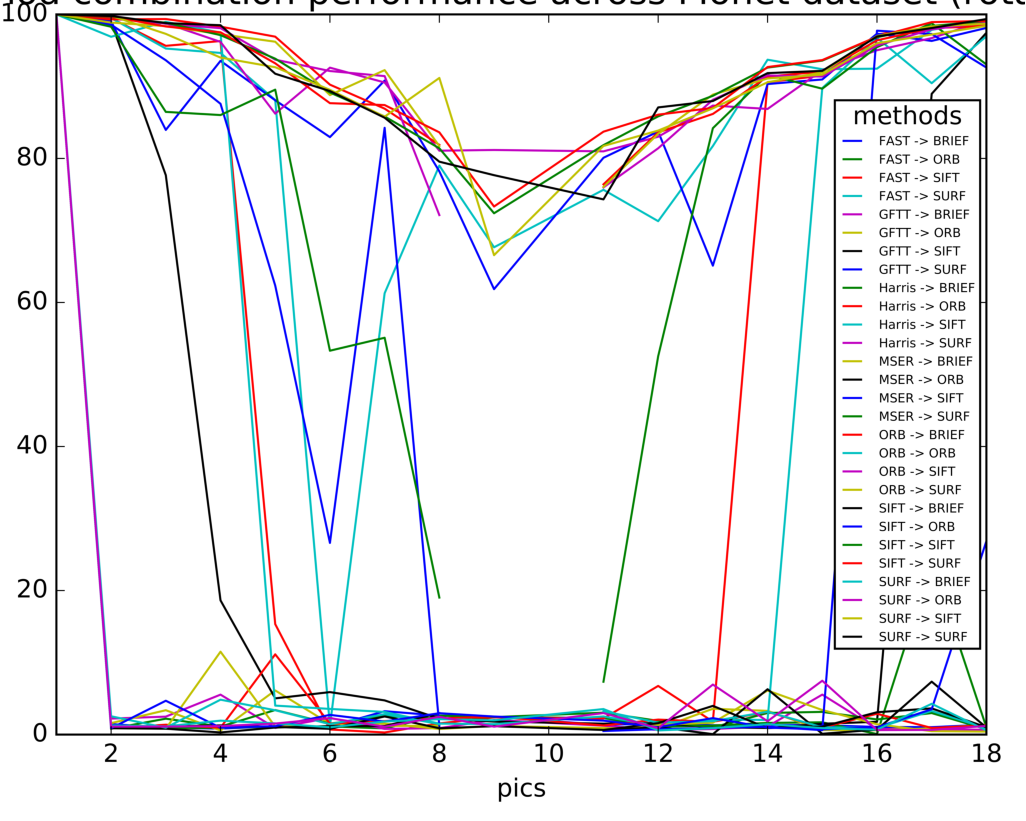
\includegraphics[scale=0.8]{text_img/graph_monet.pdf}}
	\caption{Kvalita odhadu homografie na párech obrázků ze subsetu monet (rotace)}
\end{figure}

\begin{figure}[htp] 
	\label{graph_asterix}
	\centering{
		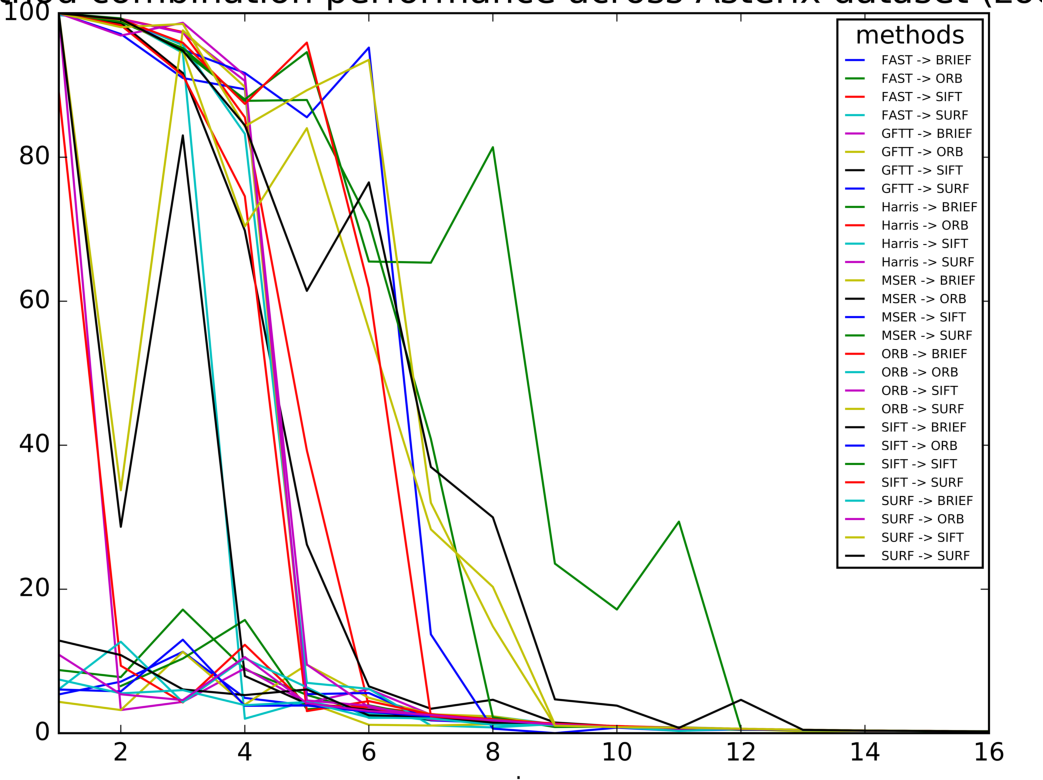
\includegraphics[scale=0.8]{text_img/graph_asterix.pdf}}
	\caption{Kvalita odhadu homografie na párech obrázků ze subsetu asterix (zoom)}
\end{figure}